% !TEX root = main.tex

% Common Styles

\def\anonymous{0}
\def\cameraready{1}
\def\fullversion{2}

\def\article{0}
\def\lncs{1}
\def\sigalternate{2}
\def\usenix{3}
\def\ieeetr{4}
\def\sciendo{5}
\def\lipics{6}

\PassOptionsToPackage{protrusion=true, expansion, tracking, kerning, spacing}{microtype}
\PassOptionsToPackage{usenames,dvipsnames,table}{xcolor}

% article
\ifnum\style=\article
	\documentclass[10pt,A4,headings=standardclasses,numbers=noenddot]{scrartcl}
	\usepackage{amsmath,amsfonts,amssymb,amsthm}
	\usepackage{fullpage}
    \usepackage[backend=bibtex,style=alphabetic]{biblatex}
	\newtheorem{theorem}{Theorem}[section]
	\newtheorem{definition}[theorem]{Definition}
	\newtheorem{remark}{Remark}
	% \newtheorem{proof}{Proof}
	\newtheorem{lemma}{Lemma}
	\newtheorem{proposition}{Proposition}
	\newtheorem{corollary}{Corollary}
	\newtheorem{claim}{Claim}
	\newtheorem{construction}{Construction}
	\let\oldproof\proof
	\let\oldendproof\endproof
	\renewenvironment{proof}{
	\oldproof
	}{\pushQED{\qed}\oldendproof}


	\AtBeginDocument{
		\makeatletter
		\hypersetup{
    pdftitle = {\@title},
    pdfauthor = {\@author}
  	}
		\makeatother
	}
\fi

% lncs
\ifnum\style=\lncs
	\let\accentvec\vec % countermeasure against "unable to redefine math accent \vec
	\documentclass[runningheads,a4paper]{styles/llncs}
	\usepackage{amssymb}
	\usepackage{expl3}

	\let\spvec\vec % countermeasure
	\let\vec\accentvec % countermeasure
	%
	\newcommand\addbibresource[1]{
	 	\newcommand\bibfiles{#1}
	}
    \ifnum\paperversion=\fullversion
        \usepackage{fullpage}
    \fi
	% \newcommand\printbibliography{
	% 	\ifnum\paperversion=\fullversion
	% 				\bibliographystyle{alpha}
	% 	\else
	% 				\bibliographystyle{splncs04}
	% 	\fi
	% 	\bibliography{\bibfiles}
	% }
\fi

% sigalternate
\ifnum\style=\sigalternate
    \ifnum\paperversion=\anonymous
        \documentclass[sigconf,anonymous,natbib=false]{acmart}
        \settopmatter{printacmref=false, printccs=false, printfolios=true} % We want page numbers on submissions
        \setcopyright{none}
        \renewcommand\footnotetextcopyrightpermission[1]{}
    \fi
    \ifnum\paperversion=\cameraready
        \documentclass[sigconf,natbib=false]{acmart}
        \setcopyright{acmlicensed}
        \copyrightyear{2019}
        \acmYear{2019}
        \acmConference[CCS '19]{2019 ACM SIGSAC Conference on Computer and Communications Security}{November 11--15, 2019}{London, United Kingdom}
        \acmBooktitle{2019 ACM SIGSAC Conference on Computer and Communications Security (CCS '19), November 11--15, 2019, London, United Kingdom}
        \acmPrice{15.00}
        \acmDOI{xxx}
        \acmISBN{xxx}
    \fi
    \ifnum\paperversion=\fullversion
        \documentclass[sigconf,natbib=false]{acmart}
        \settopmatter{printacmref=false, printccs=false, printfolios=true} % We want page numbers on full versions
        \setcopyright{none}
        \renewcommand\footnotetextcopyrightpermission[1]{}
    \fi
	%\usepackage[keeplastbox]{flushend}
	\clubpenalty=10000
	\widowpenalty = 10000
	%using the coding \vfill\eject just before the section head code will
	%force over the head to the next page or column to help rectify the
	%bad break.
	\newtheorem{remark}{Remark}
    \usepackage[
    backend=bibtex,
    style=ACM-Reference-Format
    ]{biblatex}
\fi

% usenix
\ifnum\style=\usenix
	\documentclass[letterpaper,twocolumn,10pt]{article}
	% Let LaTeX think cite is already loaded
	\usepackage{styles/usenix}
	\usepackage{epsfig}
	\usepackage{amsmath,amsfonts, amssymb, amsthm}
	%\usepackage{endnotes}
	\newtheorem{theorem}{Theorem}[section]
	\newtheorem{definition}[theorem]{Definition}
	\newtheorem{remark}{Remark}
	\newtheorem{lemma}{Lemma}
	\let\oldproof\proof
	\let\oldendproof\endproof
	\renewenvironment{proof}{
	\oldproof
	}{\pushQED{\qed}\oldendproof}
	\usepackage[
    backend=bibtex,
    style=numeric
    ]{biblatex} % Need to comment out \usepackage{cite} in usenix.sty
	\DeclareMathAlphabet{\mathcal}{OMS}{cmsy}{m}{n}
\fi

% ieeetr
\ifnum\style=\ieeetr
	\documentclass[compsoc, conference, letterpaper, 10pt, times]{styles/IEEEtran}
	\IEEEoverridecommandlockouts
    \def\BibTeX{{\rm B\kern-.05em{\sc i\kern-.025em b}\kern-.08em
            T\kern-.1667em\lower.7ex\hbox{E}\kern-.125emX}}
		\newtheorem{theorem}{Theorem}[section]
    \newtheorem{definition}[theorem]{Definition}
    \newtheorem{remark}{Remark}
    \newtheorem{proof}{Proof}
    \newtheorem{lemma}{Lemma}
    \usepackage[style=ieee,backend=bibtex]{biblatex}
\fi

% DeGryuter (PETS)
\ifnum\style=\sciendo
\documentclass[USenglish,oneside,twocolumn]{article}
\PassOptionsToPackage{english}{babel}
% Disabled natbib in dgruyter_NEW as it was annoying
\usepackage[big]{styles/dgruyter_NEW} %Contains amsmath, amssymb, authblk, multicol, graphicx, babel,  inter alia
\usepackage{amsfonts,amsthm}
\usepackage[
style=numeric-comp,
backend=bibtex8,
maxbibnames=99,
natbib=true,
maxcitenames=6,
giveninits=true,
]{biblatex}
\cclogo{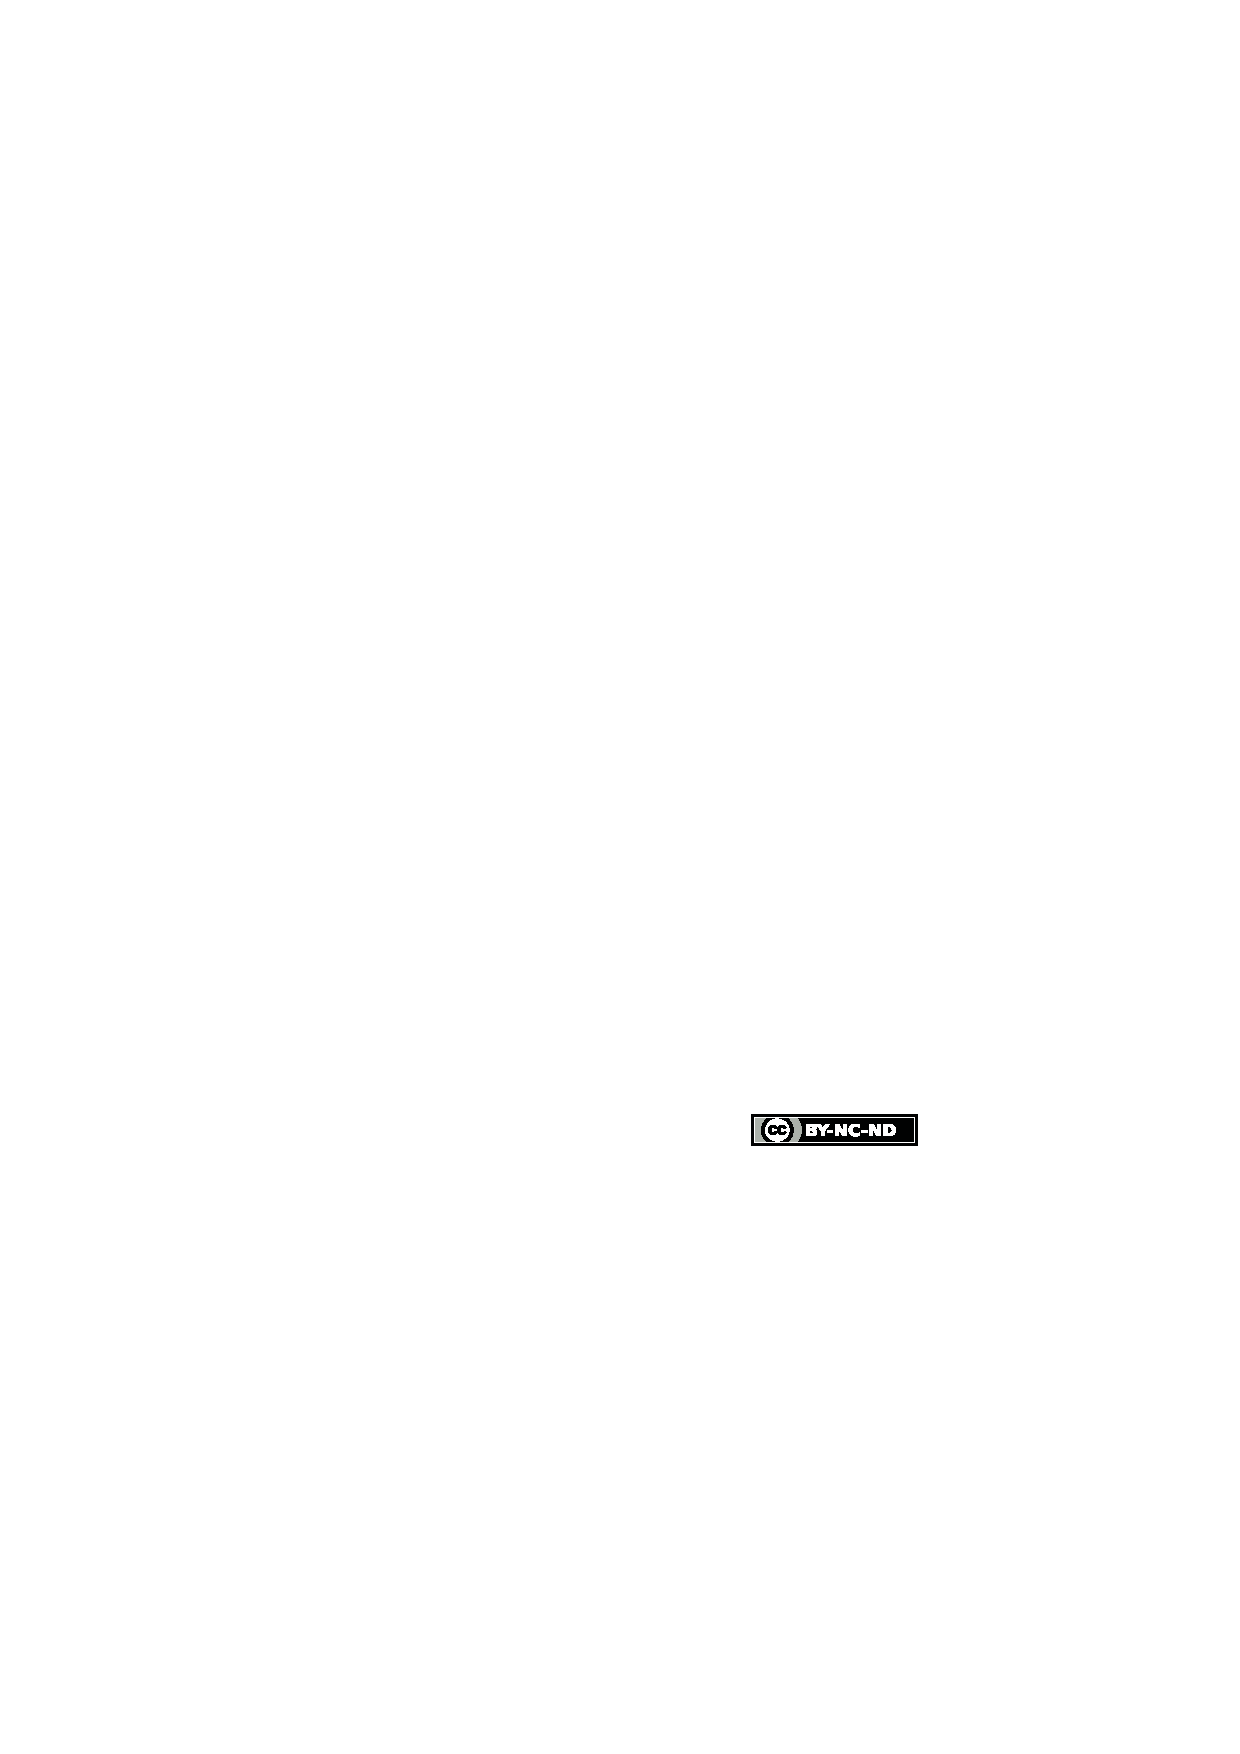
\includegraphics{styles/by-nc-nd.pdf}}

\newtheorem{theorem}{Theorem}[section]
\newtheorem{definition}[theorem]{Definition}
\newtheorem{remark}{Remark}
\newtheorem{lemma}{Lemma}
\fi

% LIPIcs
\ifnum\style=\lipics
\ifnum\paperversion=\anonymous
\documentclass[a4paper,UKenglish,numberwithinsect,thm-restate,anonymous]{styles/lipics-v2019}
\else
\documentclass[a4paper,UKenglish,numberwithinsect,thm-restate]{styles/lipics-v2019}
\fi
\PassOptionsToPackage{english}{babel}

\newcommand\printbibliography{
  \bibliographystyle{plainurl}% the mandatory bibstyle
  \bibliography{\bibfiles}
}



\newcommand\addbibresource[1]{
  \newcommand\bibfiles{#1}
}

\fi



%%% For compatibility to BibTex
%	\newcommand\addbibresource[1]{
%		\newcommand\bibfiles{#1}
%	}
%	\newcommand\printbibliography{
%		\bibliography{\bibfiles}
%	}

%%% Local Variables:
%%% mode: latex
%%% TeX-master: "main"
%%% End:
